The NOMP, MUSIC, and LASSO algorithms all have very promising results, however they are computationally complex. The calculation of CSI and channel estimation are done frequently due to constantly changing channel conditions. Channel estimation algorithms have a real-time constraint, the faster they are the more accurate the results and the longer they will be relevant. For this reason, path estimation is a problem that could be solved using a Machine Learning (ML) algorithm. Often trained models can solve a complex problem with a faster run time than traditional algorithms. The authors of \cite{Li2020} represent the sparse channel as an image and use a the YOLO algorithm to identify the dominant paths. With reasonably good SNR ratios, the delay-angle transform produces an image with very pronounced paths. It is possible that a more basic image recognition algorithm may outperform YOLO in run time without sacrificing the accuracy. Additionally, the authors require sparsity for their algorithm to function, it is possible that different ML algorithms may not require channel sparsity. 

This project will be an analysis of m-MIMO path estimation techniques with a focus on run time and performance. This will require a m-MIMO simulator to create realistic channel data along with received and transmitted pilots. It
will include an implementation of one or more classical algorithms such as NOMP, LASSO, or MUSIC, as well as the YOLO algorithm described in \cite{Li2020}. New ML and classical image processing algorithms will be compared with the state of the art under varying channel conditions. The results will be presented in a report assessing the which techniques are the most practical for path gain delay and angle estimation.





% Comments out a block
\iffalse
Objectives
\begin{itemize}
    \item Creation of a m-MIMO simulation
    \item Reproduce results from \cite{Li2020}
    \item Improve deep learning algorithm or introduce a new machine learning model
    \item Investigate other estimation techniques
    \item Argue and present evidence for the best technique
\end{itemize}
\fi

\iffalse
\begin{wrapfigure}{l}{0.25\textwidth}
    \centering
    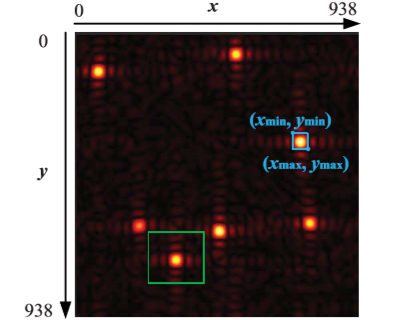
\includegraphics[width=0.3\textwidth]{YOLO.png}
\end{wrapfigure}


First, we will make a m-MIMO simulator using MATLAB toolboxes. The simulator will use a Clustered Delay Line (CDL) channel model from the 5G toolbox \cite{matlab}. The channel model allows us to randomize the channel parameters and apply its affects to pilot symbols. Additionally, the toolbox has functions to calculate the CSI. The output of the simulation will be the CSI, along with the transmitted and received pilots, which will be stored in a data set. Next, we will use this data set to reproduce the results in \cite{Li2020}. This involves implementing a traditional algorithm such as NOMP and the YOLO based method. Finally, we plan to test different image processing algorithms to compare their speed and accuracy to the methods shown in \cite{Li2020}.
\fi